\documentclass[a4]{article}
\pagestyle{myheadings}

%%%%%%%%%%%%%%%%%%%
% Packages/Macros %
%%%%%%%%%%%%%%%%%%%
\usepackage{mathrsfs}


\usepackage{fancyhdr}
\pagestyle{fancy}
\lhead{}
\chead{}
\rhead{}
\lfoot{}
\cfoot{} 
\rfoot{\normalsize\thepage}
\renewcommand{\headrulewidth}{0pt}
\renewcommand{\footrulewidth}{0pt}
\newcommand{\RomanNumeralCaps}[1]
    {\MakeUppercase{\romannumeral #1}}

\usepackage{amssymb,latexsym}  % Standard packages
\usepackage[utf8]{inputenc}
\usepackage[russian]{babel}
\usepackage{MnSymbol}
\usepackage{mathrsfs}
\usepackage{amsmath,amsthm}
\usepackage{indentfirst}
\usepackage{graphicx}%,vmargin}
\usepackage{graphicx}
\graphicspath{{pictures/}} 
\usepackage{verbatim}
\usepackage{color}
\usepackage[nottoc,numbib]{tocbibind}
\usepackage{float}

\usepackage{listings}
\definecolor{codegreen}{rgb}{0,0.6,0}
\definecolor{codegray}{rgb}{0.5,0.5,0.5}
\definecolor{codepurple}{rgb}{0.58,0,0.82}
\definecolor{backcolour}{rgb}{0.95,0.95,0.92}
 
\lstdefinestyle{mystyle}{
    backgroundcolor=\color{backcolour},   
    commentstyle=\color{codegreen},
    keywordstyle=\color{magenta},
    numberstyle=\tiny\color{codegray},
    stringstyle=\color{codepurple},
    basicstyle=\footnotesize,
    breakatwhitespace=false,         
    breaklines=true,                 
    captionpos=b,                    
    keepspaces=true,                 
    numbers=left,                    
    numbersep=5pt,                  
    showspaces=false,                
    showstringspaces=false,
    showtabs=false,                  
    tabsize=2
}
 
\lstset{style=mystyle}

\usepackage{url}
\urldef\myurl\url{foo%.com}





\DeclareGraphicsExtensions{.pdf,.png,.jpg}% -- настройка картинок

\usepackage{epigraph} %%% to make inspirational quotes.
\usepackage[all]{xy} %for XyPic'a
\usepackage{color} 
\usepackage{amscd} %для коммутативных диграмм
%\usepackage[colorlinks,urlcolor=red]{hyperref}

%\renewcommand{\baselinestretch}{1.5}
%\sloppy
%\usepackage{listings}
%\lstset{numbers=left}
%\setmarginsrb{2cm}{1.5cm}{1cm}{1.5cm}{0pt}{0mm}{0pt}{13mm}


\newtheorem{Lemma}{Лемма}[section]
\newtheorem{Proposition}{Предложение}[section]
\newtheorem{Theorem}{Теорема}[section]
\newtheorem{Corollary}{Следствие}[section]
\newtheorem{Remark}{Замечание}[section]
\newtheorem{Definition}{Определение}[section]
\newtheorem{Designations}{Обозначение}[section]




%%%%%%%%%%%%%%%%%%%%%%% 
%Подготовка оглавления% 
%%%%%%%%%%%%%%%%%%%%%%% 
\usepackage[titles]{tocloft}
\renewcommand{\cftdotsep}{2} %частота точек
\renewcommand\cftsecleader{\cftdotfill{\cftdotsep}}
\renewcommand{\cfttoctitlefont}{\hspace{0.38\textwidth} \LARGE\bfseries} 
\renewcommand{\cftsecaftersnum}{.}
\renewcommand{\cftsubsecaftersnum}{.}
\renewcommand{\cftbeforetoctitleskip}{-1em} 
\renewcommand{\cftaftertoctitle}{\mbox{}\hfill \\ \mbox{}\hfill{\footnotesize Стр.}\vspace{-0.5em}} 
%\renewcommand{\cftchapfont}{\normalsize\bfseries \MakeUppercase{\chaptername} } 
%\renewcommand{\cftsecfont}{\hspace{1pt}} 
\renewcommand{\cftsubsecfont}{\hspace{1pt}} 
%\renewcommand{\cftbeforechapskip}{1em} 
\renewcommand{\cftparskip}{3mm} %определяет величину отступа в оглавлении
\setcounter{tocdepth}{5} 
\renewcommand{\listoffigures}{\begingroup %добавляем номер в список иллюстраций
\tocsection
\tocfile{\listfigurename}{lof}
\endgroup}
\renewcommand{\listoftables}{\begingroup %добавляем номер в список иллюстраций
\tocsection
\tocfile{\listtablename}{lot}
\endgroup}


   
   
%\renewcommand{\thelikesection}{(\roman{likesection})}
%%%%%%%%%%%
% Margins %
%%%%%%%%%%%
\addtolength{\textwidth}{0.7in}
\textheight=630pt
\addtolength{\evensidemargin}{-0.4in}
\addtolength{\oddsidemargin}{-0.4in}
\addtolength{\topmargin}{-0.4in}

%%%%%%%%%%%%%%%%%%%%%%%%%%%%%%%%%%%
%%%%%%Переопределение chapter%%%%%% 
%%%%%%%%%%%%%%%%%%%%%%%%%%%%%%%%%%%
\newcommand{\empline}{\mbox{}\newline} 
\newcommand{\likechapterheading}[1]{ 
\begin{center} 
\textbf{\MakeUppercase{#1}} 
\end{center} 
\empline} 

%%%%%%%Запиливание переопределённого chapter в оглавление%%%%%% 
\makeatletter 
\renewcommand{\@dotsep}{2} 
\newcommand{\l@likechapter}[2]{{\bfseries\@dottedtocline{0}{0pt}{0pt}{#1}{#2}}} 
\makeatother 
\newcommand{\likechapter}[1]{ 
\likechapterheading{#1} 
\addcontentsline{toc}{likechapter}{\MakeUppercase{#1}}} 




\usepackage{xcolor}
\usepackage{hyperref}
\definecolor{linkcolor}{HTML}{000000} % цвет ссылок
\definecolor{urlcolor}{HTML}{AA1622} % цвет гиперссылок
 
\hypersetup{pdfstartview=FitH,  linkcolor=linkcolor,urlcolor=urlcolor, colorlinks=true}

%%%%%%%%%%%%
% Document %
%%%%%%%%%%%%

%%%%%%%%%%%%%%%%%%%%%%%%%%%%%
%%%%%%главы -- section*%%%%%%
%%%%section -- subsection%%%%
%subsection -- subsubsection%
%%%%%%%%%%%%%%%%%%%%%%%%%%%%%
\def \newstr {\medskip \par \noindent} 



\begin{document}
\def\contentsname{\LARGE{Содержание}}
\thispagestyle{empty}
\begin{center} 
\vspace{2cm} 
{\Large \sc Санкт-Петербургский Политехнический}\\
\vspace{2mm}
{\Large \sc Университет} им. {\Large\sc Петра Великого}\\
\vspace{1cm}
{\large \sc Институт прикладной математики и механики\\ 
\vspace{0.5mm}
\textsc{}}\\ 
\vspace{0.5mm}
{\large\sc Кафедра прикладной математики}\\
\vspace{15mm}
%\rule[0.5ex]{\linewidth}{2pt}\vspace*{-\baselineskip}\vspace*{3.2pt} 
%\rule[0.5ex]{\linewidth}{1pt}\\[\baselineskip] 
{\huge \sc Лабораторная работа №$2$\\
%\vspace{4mm}
%Расстояние Фреше
\vspace{6mm}
 }
\vspace*{2mm}
%\rule[0.7ex]{\linewidth}{1pt}\vspace*{-\baselineskip}\vspace{3.2pt} 
%\rule[0.5ex]{\linewidth}{2pt}\\ 
\vspace{1cm}

{\sc $4$ курс$,$ группа $3630102/60201$}

\vspace{2cm} 
Студент \hfill Д. А. Плаксин\\
\vspace{1cm}
Преподаватель \hfill Баженов А. Н.\\
\vspace{20mm} 

\end{center} 
%\author{Я}
\begin{center}
\vfill {\large\textsc{Санкт-Петербург}}\\ 
2019 г.
\end{center}

%%%%%%%%%%%%%%%%%%%%%%%%%%%%%%%%%%%%%%%%%%%%%%%%%%%%%%%%%%%%%%%%%%%%%%%%%%%%%%%%%%%%%%%%%%%%%%
%\ \\[4cm]

%\rm
%%%%%%%%%%%%%%%%%%%%%%%%%%%%%%%%%%%%%%%%%%%%%%%%%%%%%%%%%%%%%%%%%%%%%%%%%%%%%%%%%%%%%%%%%%%%%%
\newpage
\pagestyle{plain}

%\begin{center}
%\begin{abstract} 

%\end{abstract}

%\end{center}
\newpage
\tableofcontents{}
\newpage
\listoffigures{}
\newpage

\section{Постановка задачи}
Построить фигуру вращения $\--$ тор, в виде дискретного набора точек в пространстве. \hfill\cite{source}

Построить набор сечений фигуры плоскостями $x = H.$

Одно из сечений хорошо описывается лемнискатой Бернулли. Необходимо постоить лемнискату и сравнить её с соответствующим сечением.

Варьируя параметры лемнискаты и тора минимизировать расстояние (Фреше) между ними.

\section{Теория}
\subsection{Сечение тела вращения}
Сечение задаётся в плоскости $XOZ.$ Само тело получается путём вращения плоскости сечения с точками вокруг оси $Z.$ \hfill\cite{source}

Так как сечение тела представляется в виде дискретного набора точек, и каждая из точек движется по окружности, то нужно для каждой точки найти пересечение её окружности и плоскости $x = H.$ Пересечение ищется с помощью системы:
\begin{equation}
    \begin{cases}
    x^2+y^2=R^2\\
    x=H\\
    z=z'
    \end{cases}
\end{equation}

Решение системы: $(H,\pm \sqrt{R^2-H^2},z').$ Если подкоренное выражение меньше нуля, то пересечения нет.

\subsection{Лемниската Бернулли}
Параметрическое уравнение лемнискаты Бернулли: \hfill\cite{source}
\begin{equation}
    \begin{cases}
    y=c\frac{t+t^3}{1+t^4}\\
    x=c\frac{t-t^3}{1+t^4}\\
    z=z'
    \end{cases}
\end{equation}
где $t=\tg(\varphi), c\;\--$ параметр.

\section{Реализация}
Для реализации лабораторной использовался язык $Python\;3.7$. Использовалась библиотека $numpy.$\hfill\cite{numpy} 

Графики строились с помощью библиотеки $matplotlib.$ \hfill\cite{plotlib}

Трёхмерные графики строились с помощью библиотеки $mpl\_toolkits.mplot3d.$\hfill \cite{plot3}


\newpage
\section{Результаты}
\subsection{Построение сечений}
Рассматривается тор со следующими характеристиками: $R=20\;\--$ радиус вращения, $r=15\;\--$ радиус образующей.

Рассматриваемы плоскости сечения $x = H,$ где $H=\{0, 5, 10, 15, 20, 25, 35\}.$

\begin{figure}[H]
\begin{center}
\caption{Сечение тора плоскость $x=0$ }
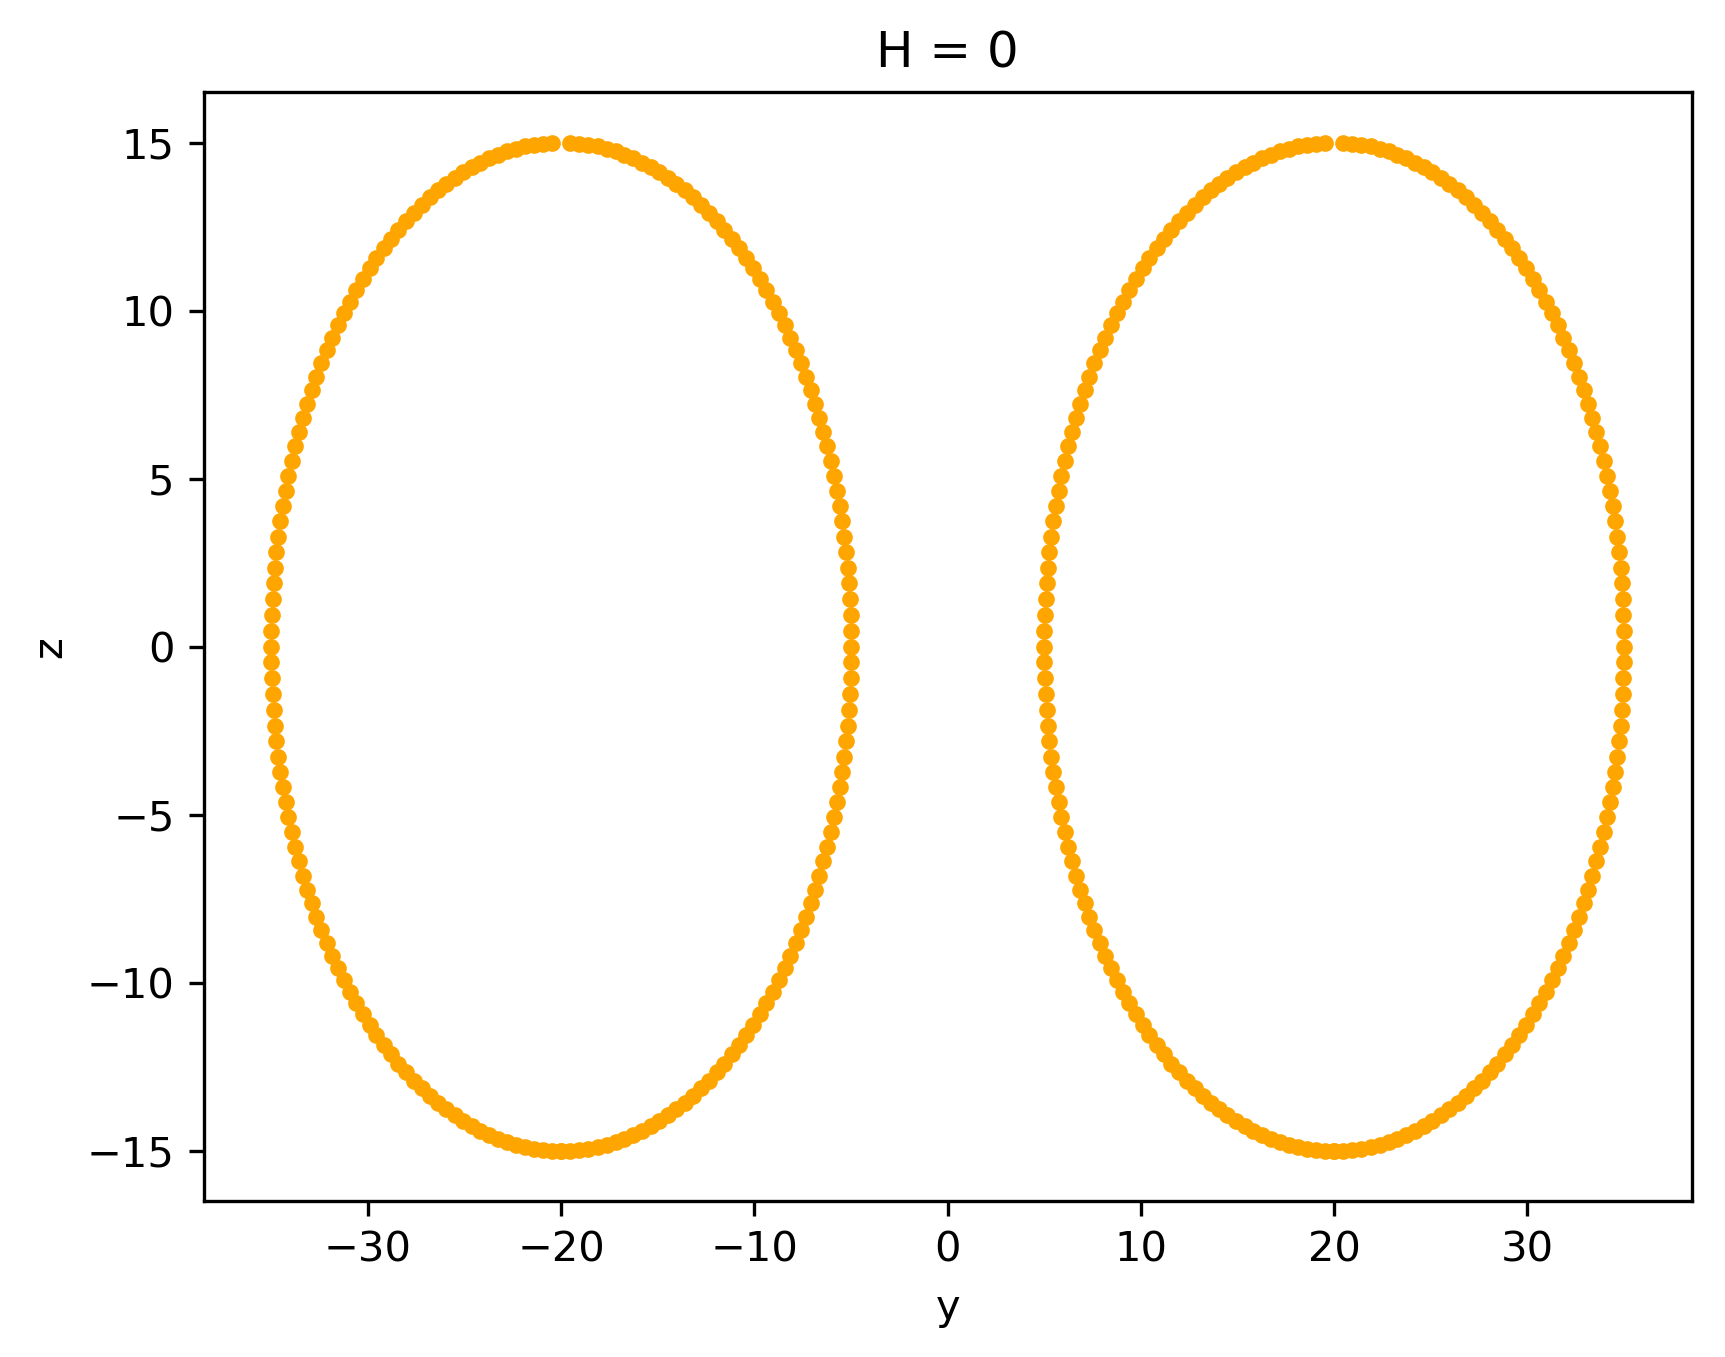
\includegraphics[scale=0.72]{TS0.png} 

\caption{Сечение тора плоскость $x=5$ }
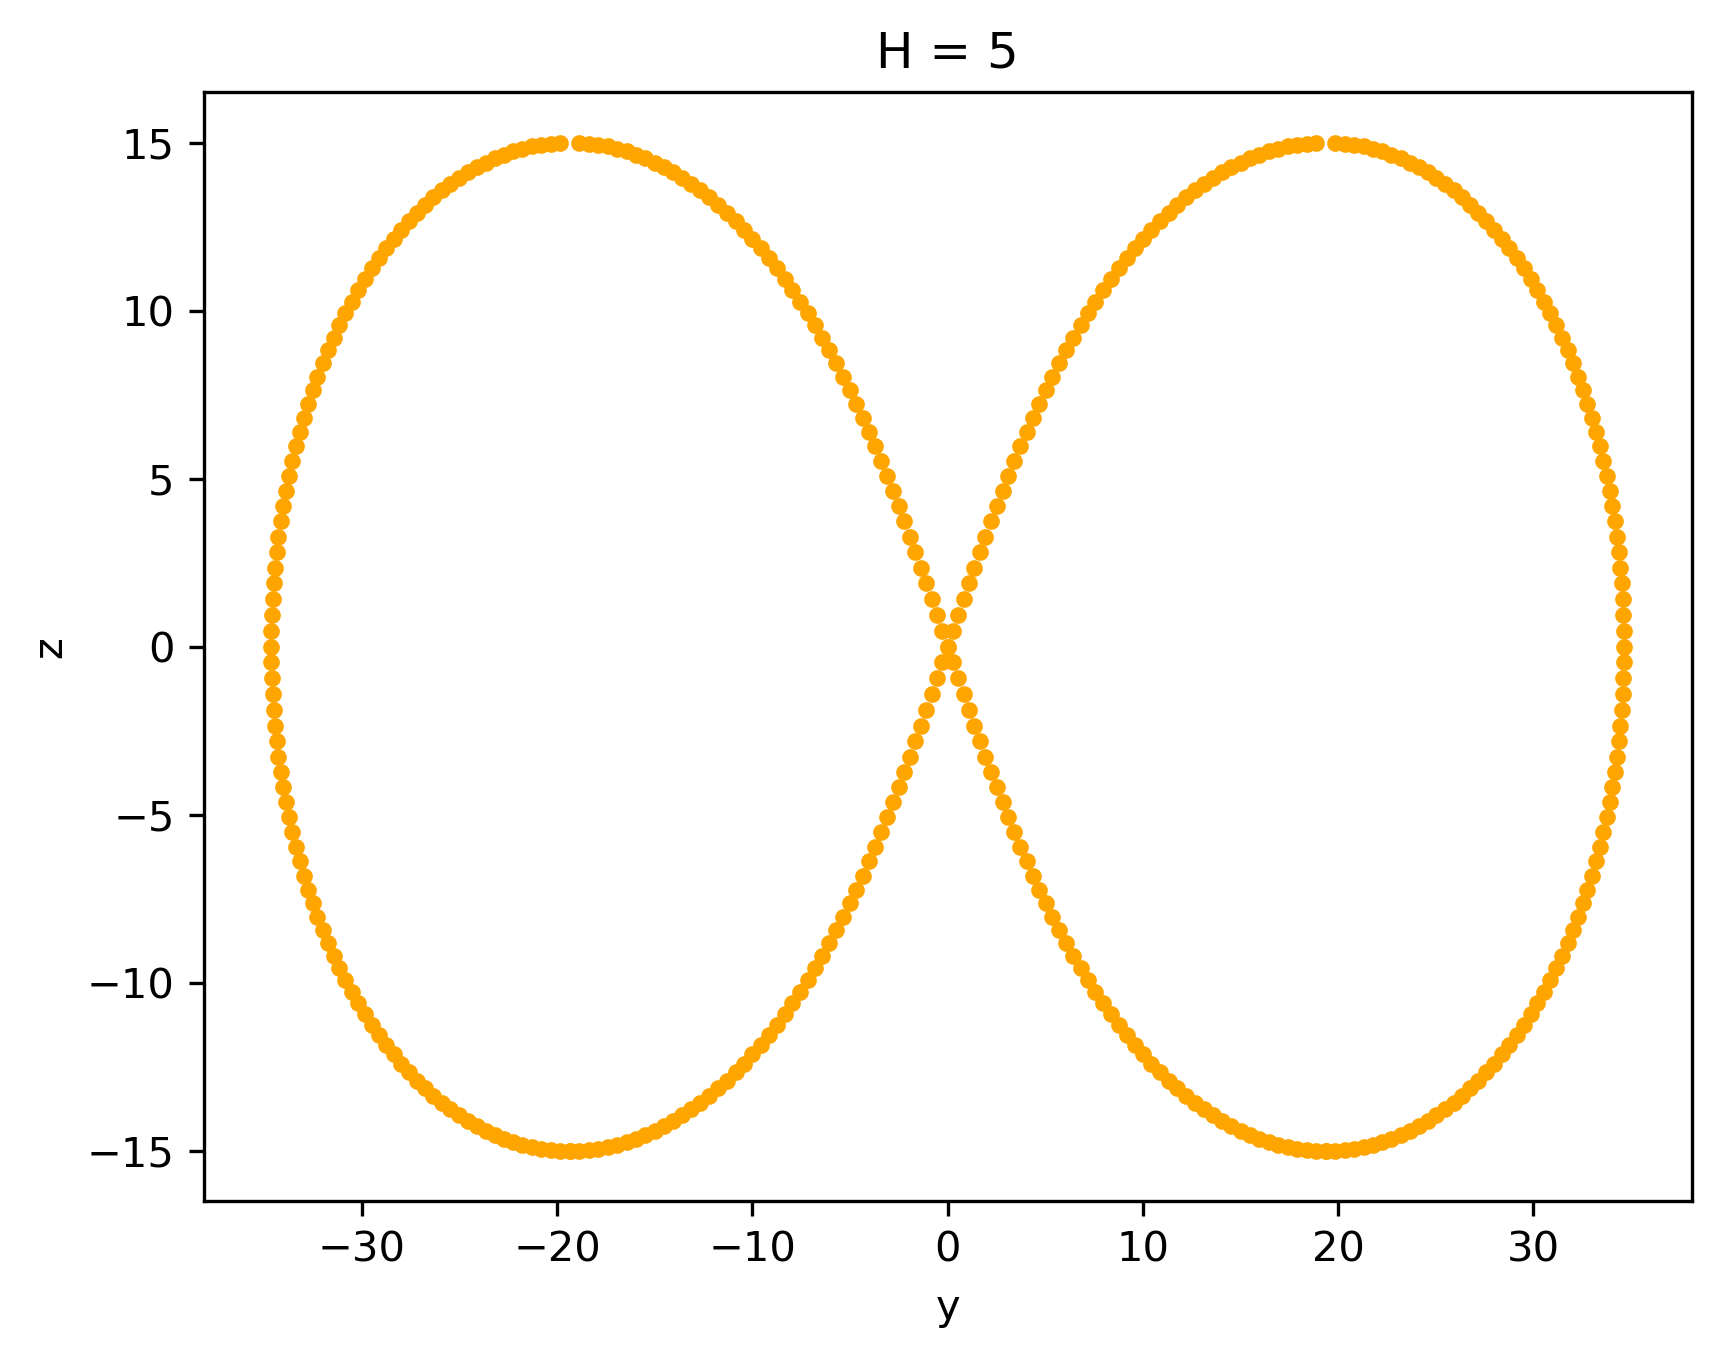
\includegraphics[scale=0.72]{TS5.png} 
\end{center}
\end{figure}


\begin{figure}[H]
\caption{Сечение тора плоскость $x=10$ }
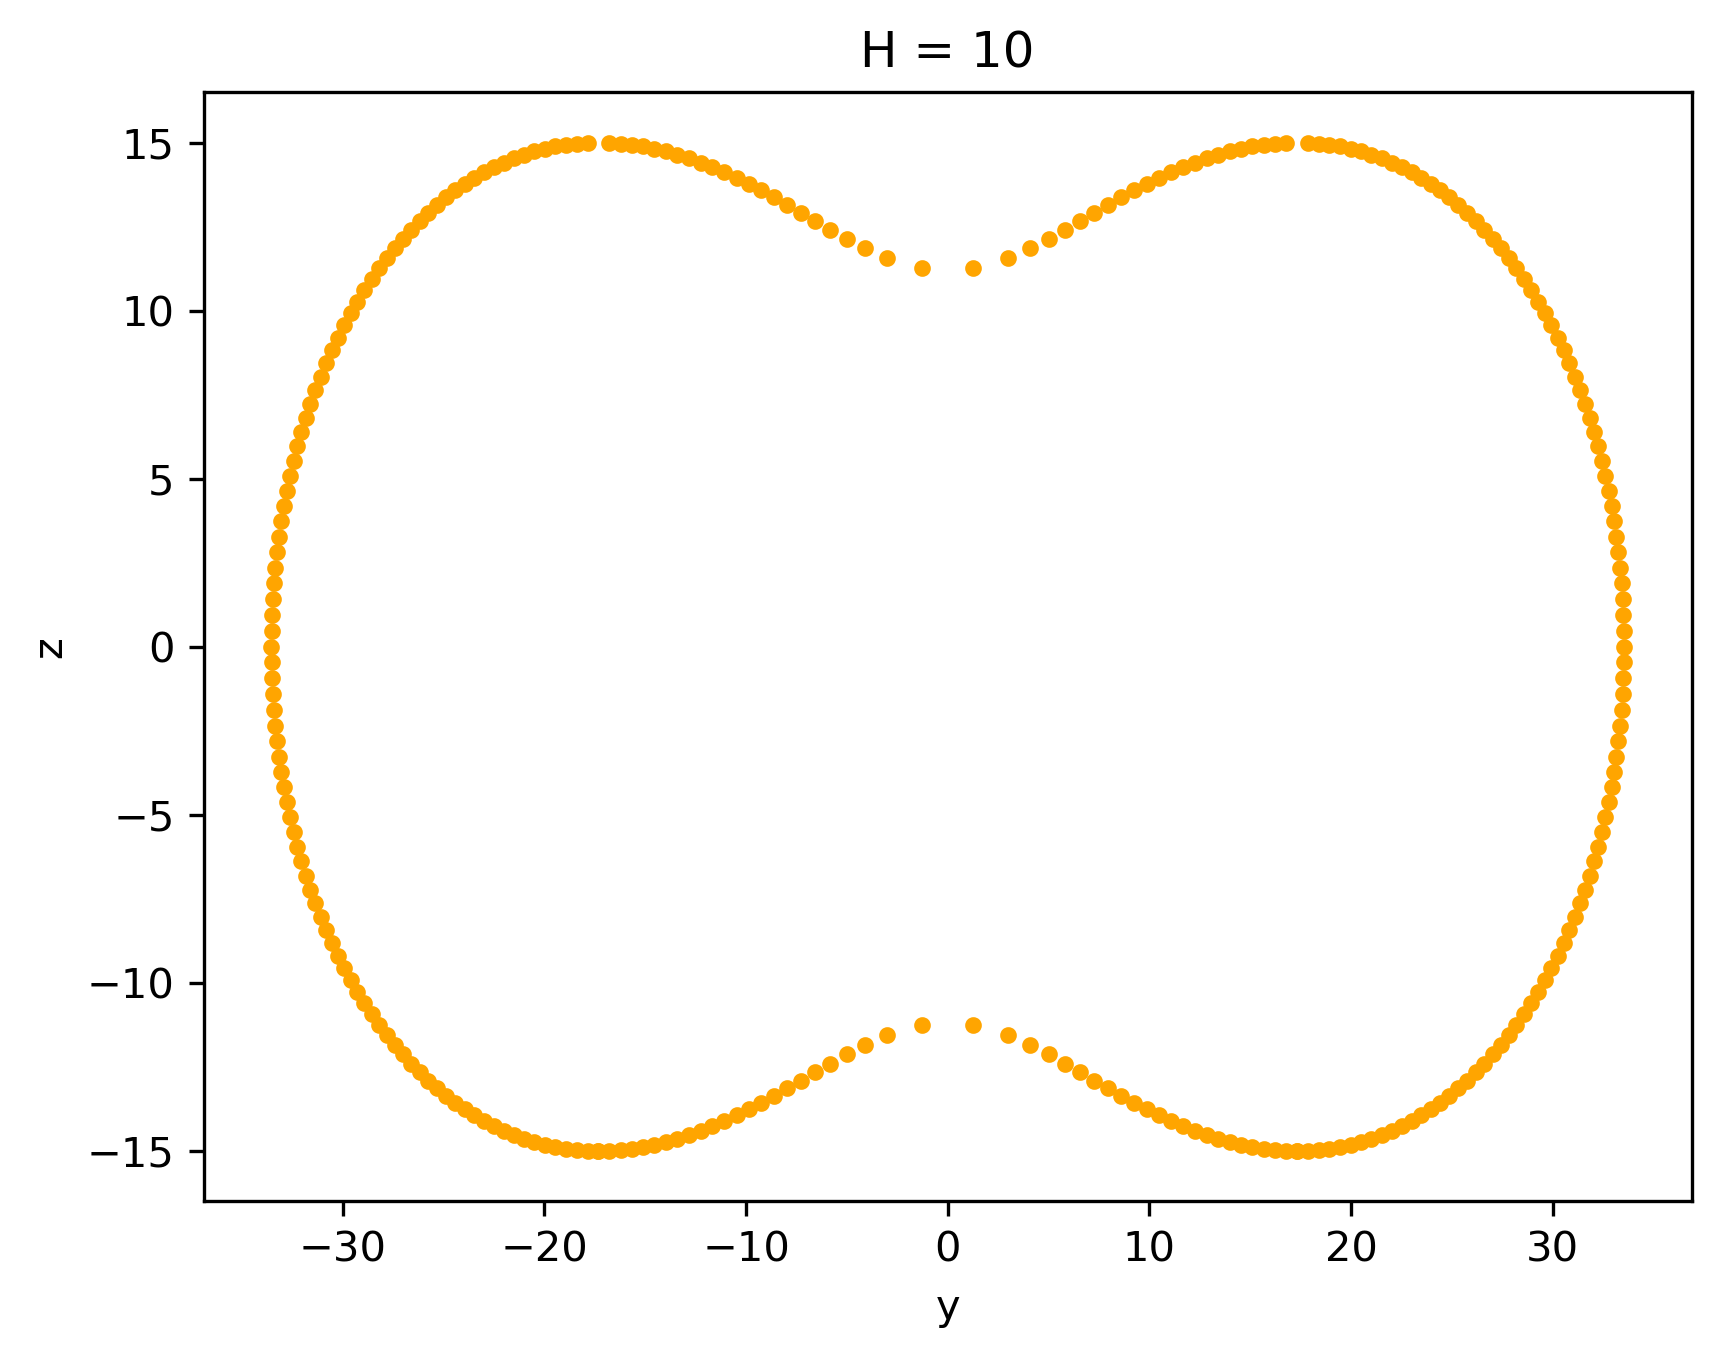
\includegraphics[scale=0.9]{TS10.png} 

\caption{Сечение тора плоскость $x=15$ }
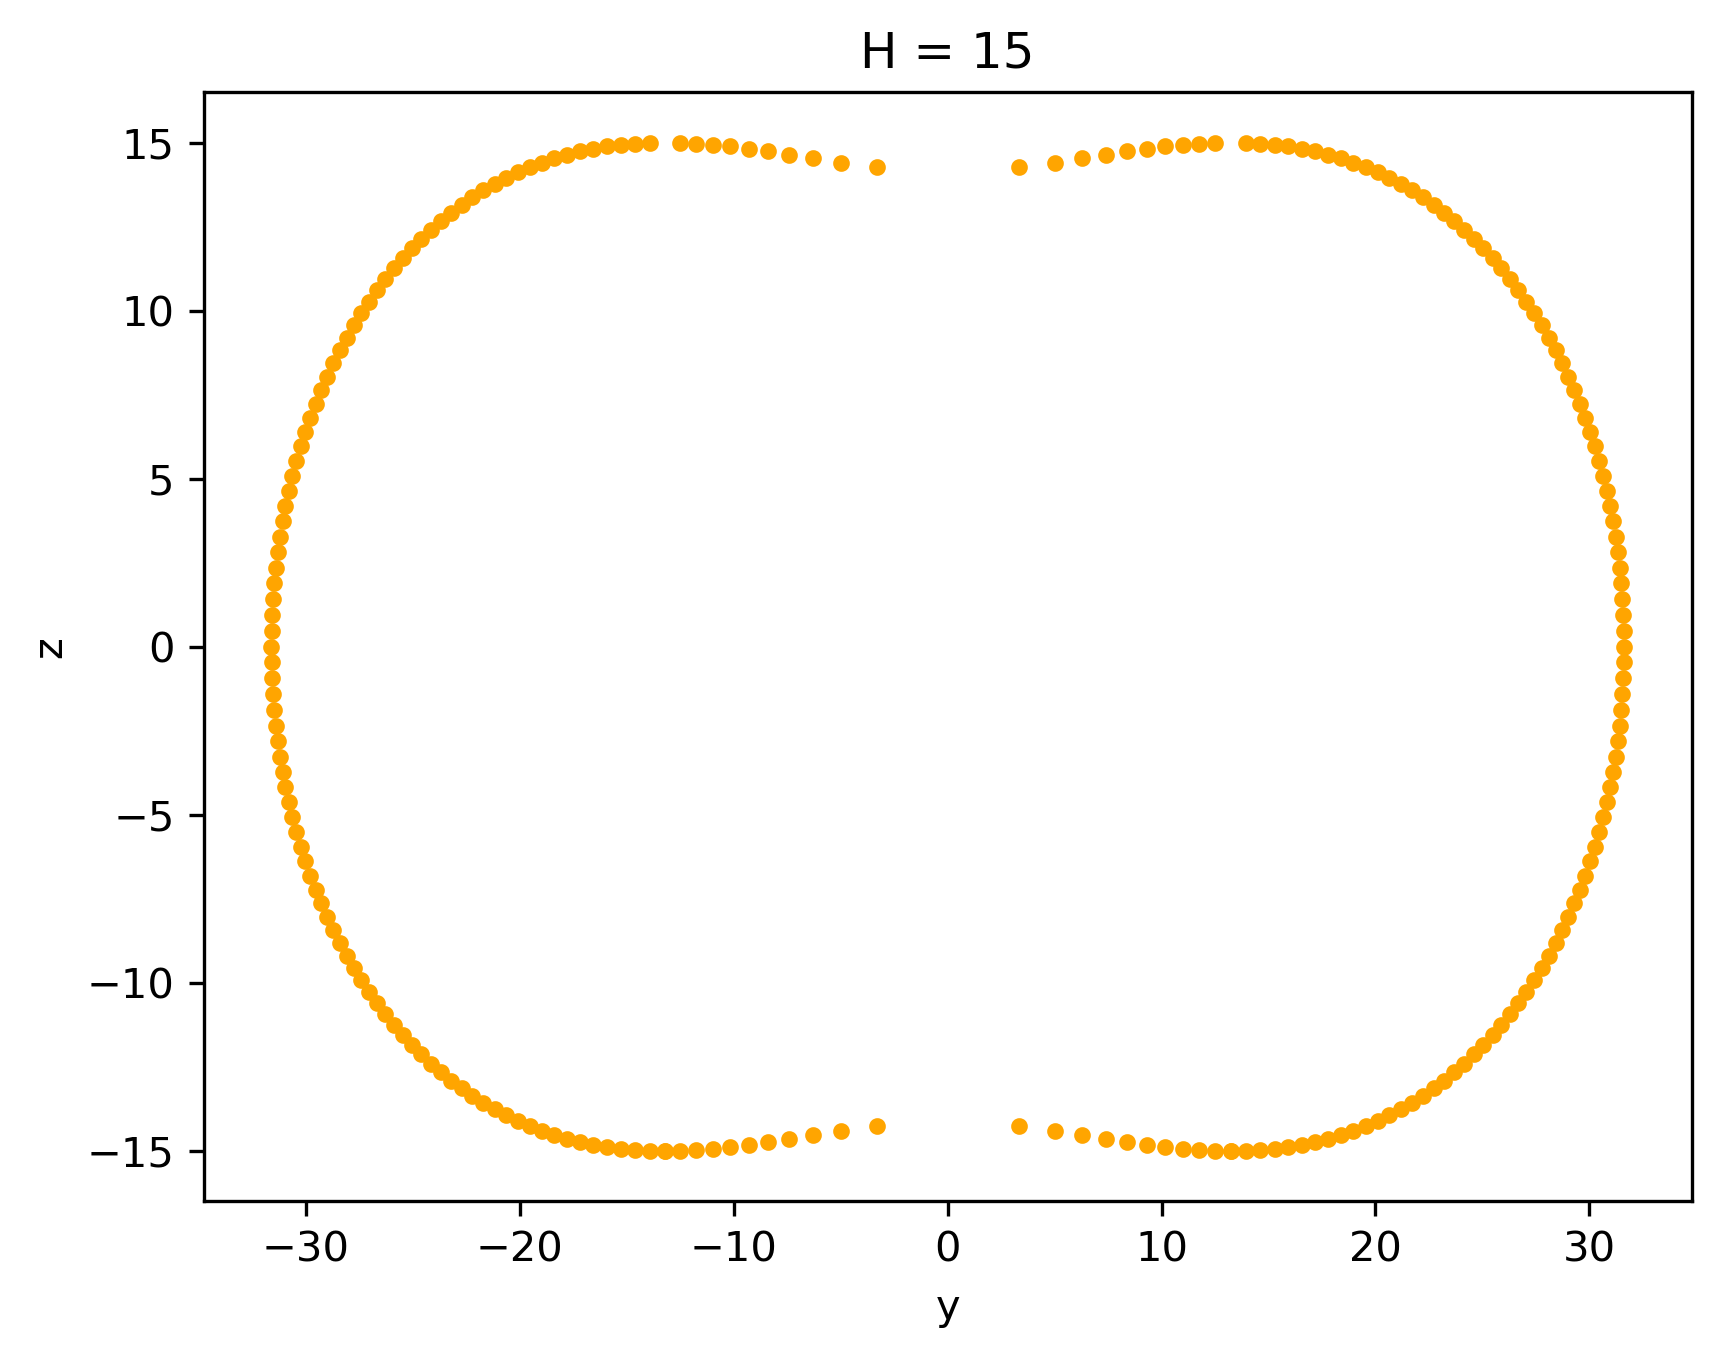
\includegraphics[scale=0.9]{TS15.png} 
\end{figure}

\begin{figure}[H]
\caption{Сечение тора плоскость $x=20$ }
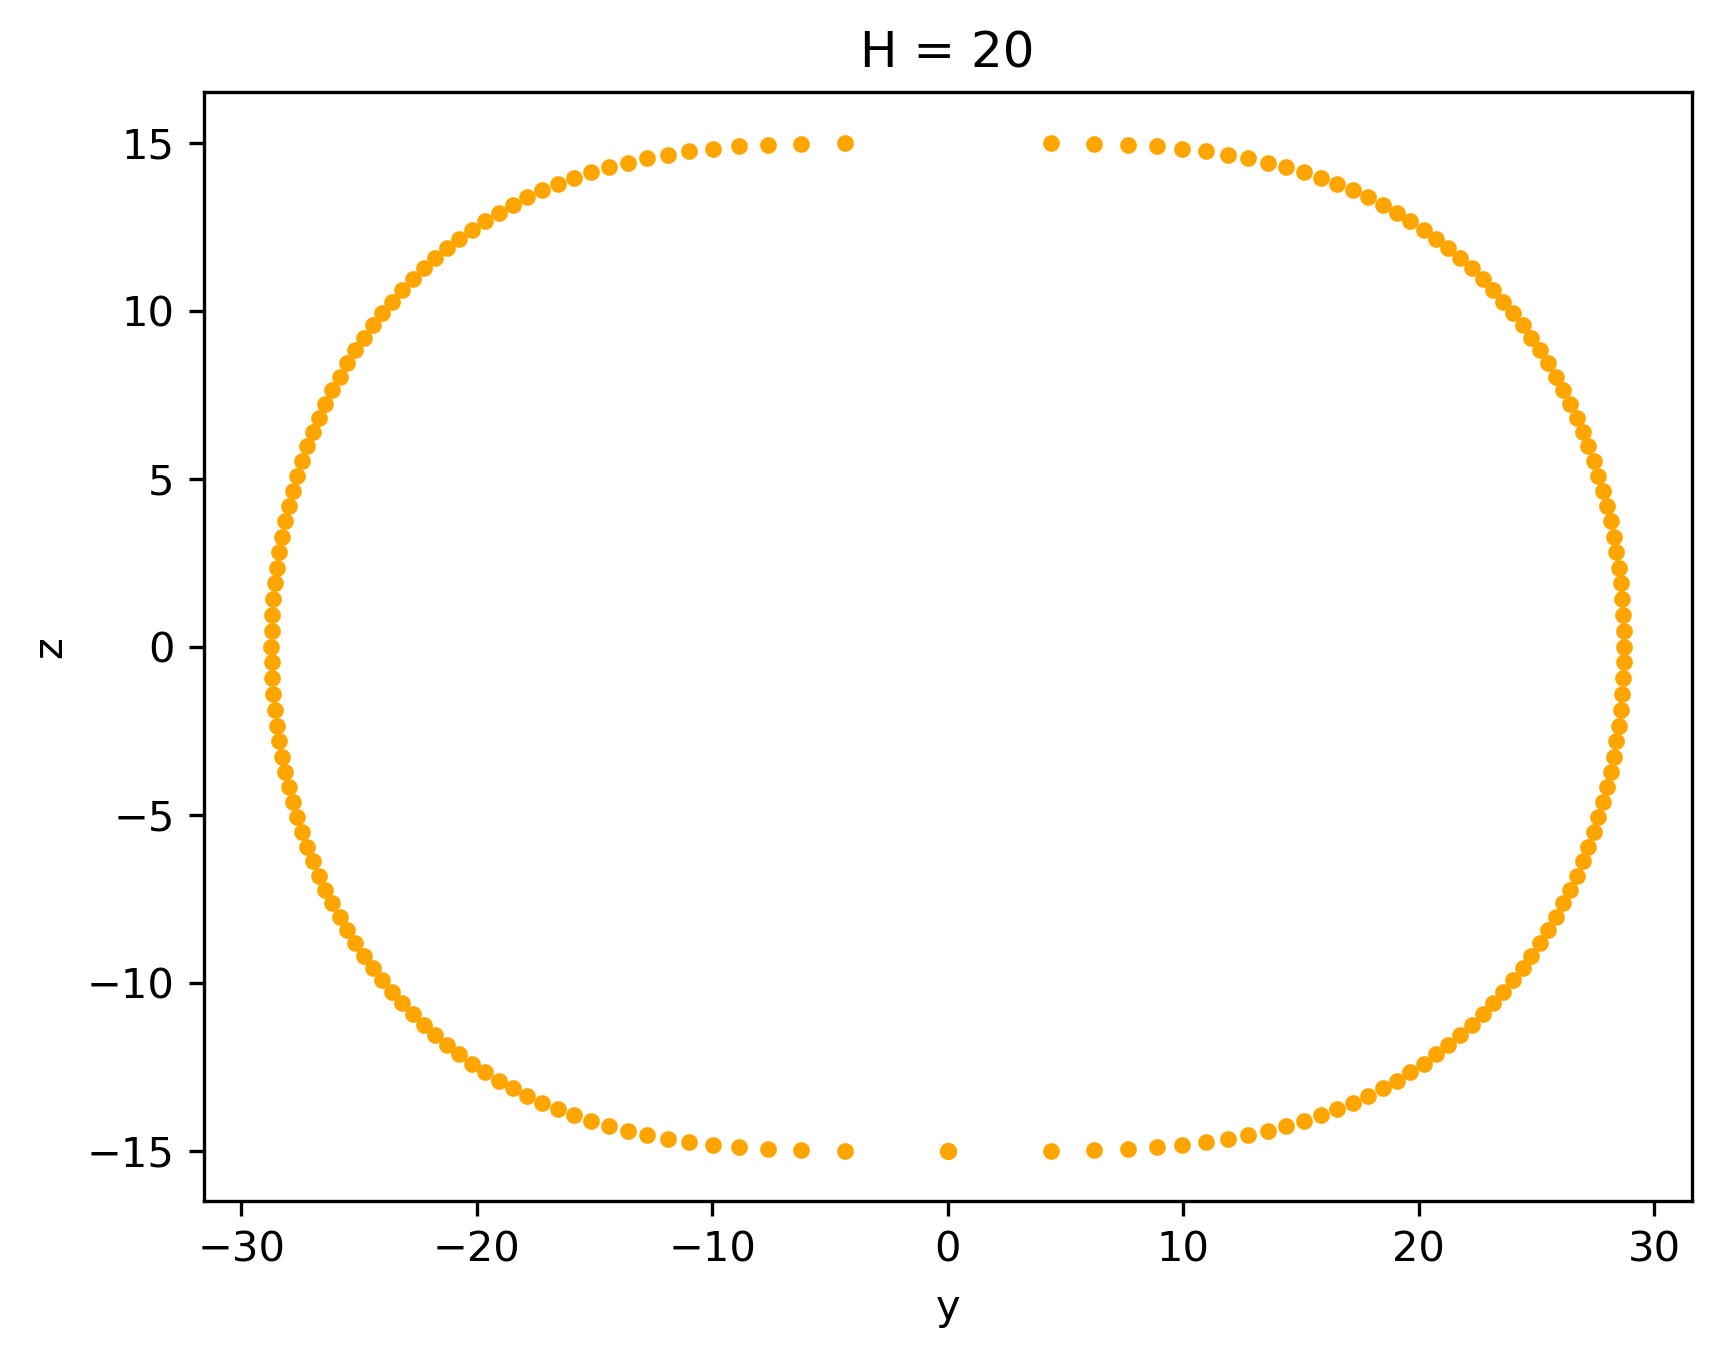
\includegraphics[scale=0.9]{TS20.png} 

\caption{Сечение тора плоскость $x=25$ }
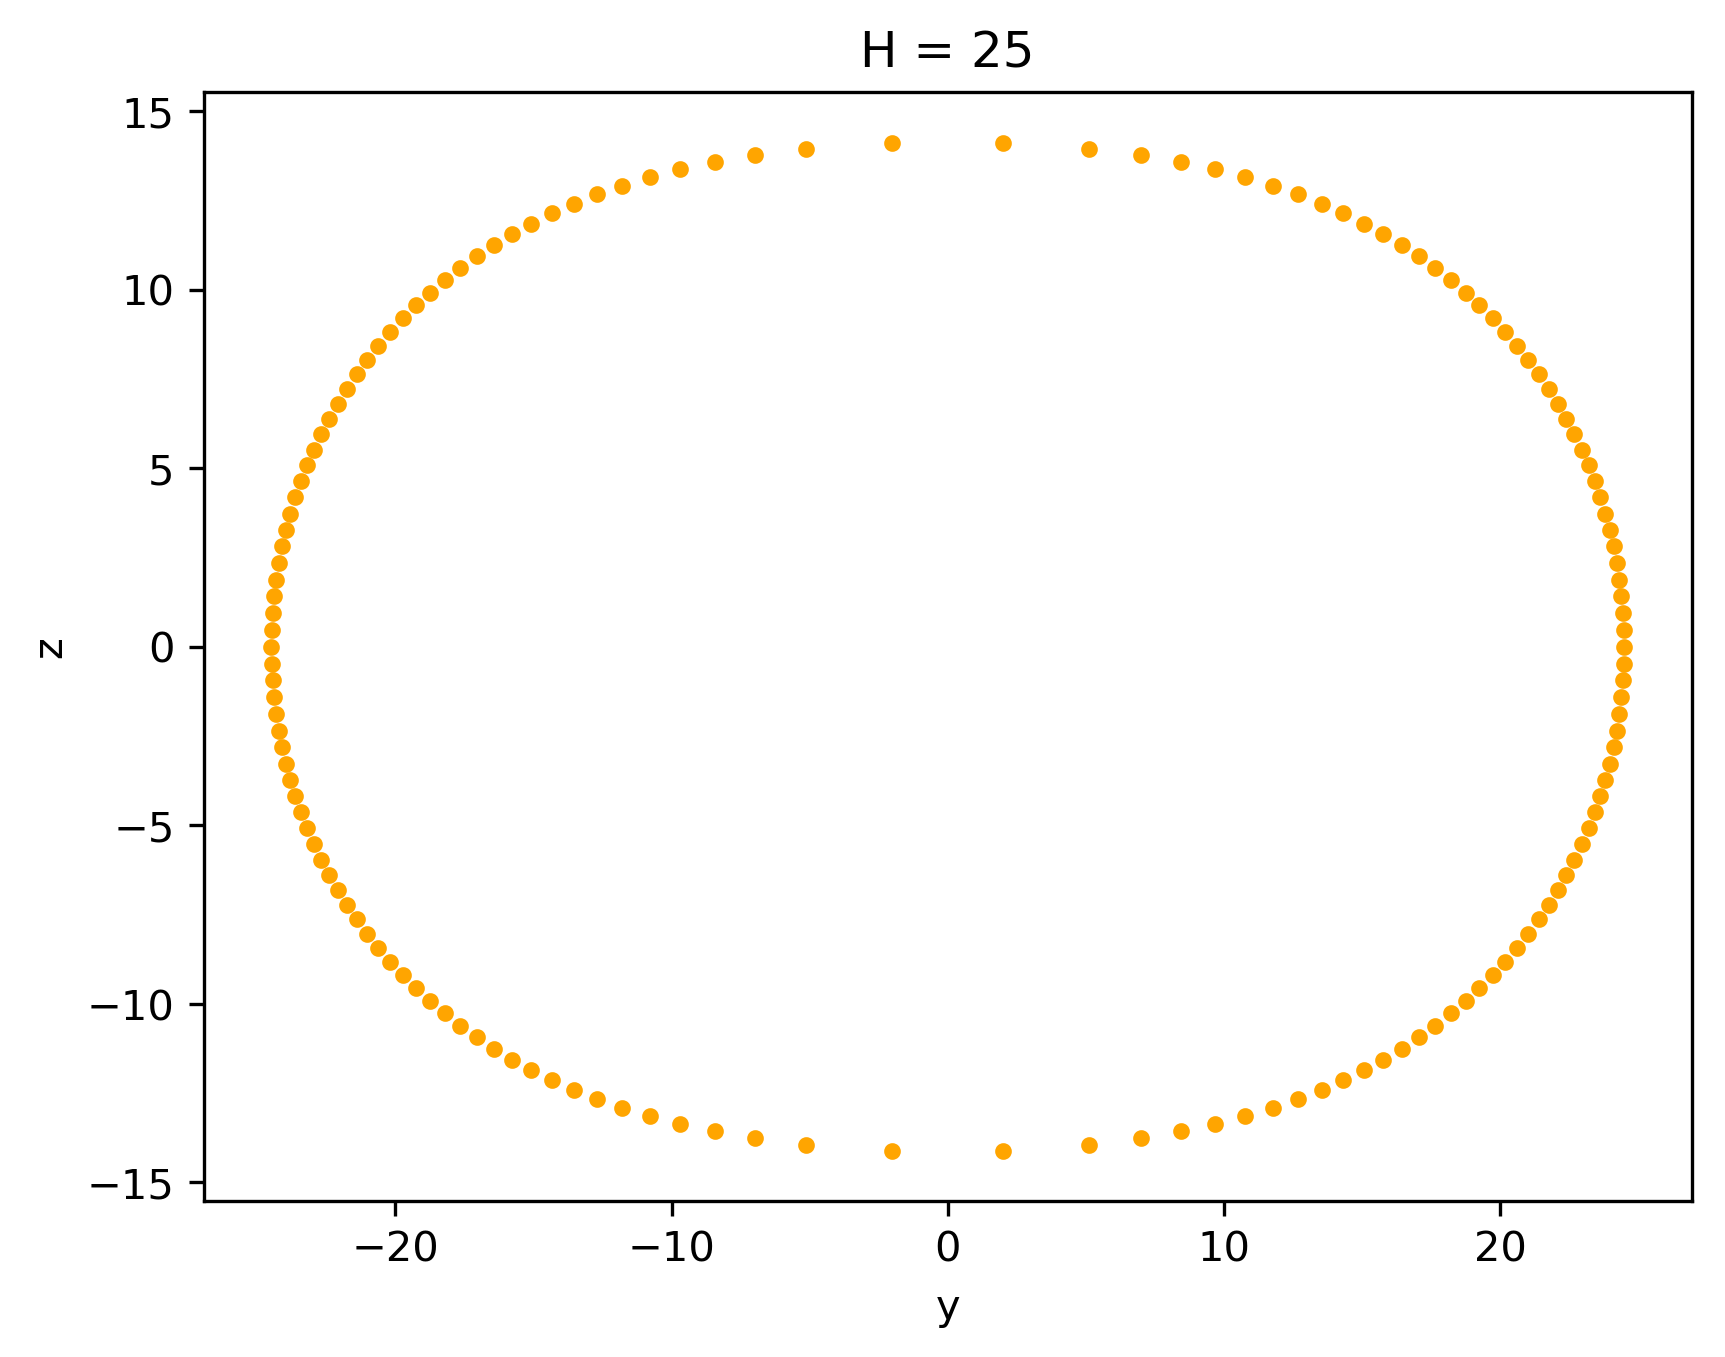
\includegraphics[scale=0.9]{TS25.png} 
\end{figure}

\begin{figure}[H]
\caption{Сечение тора плоскость $x=30$ }
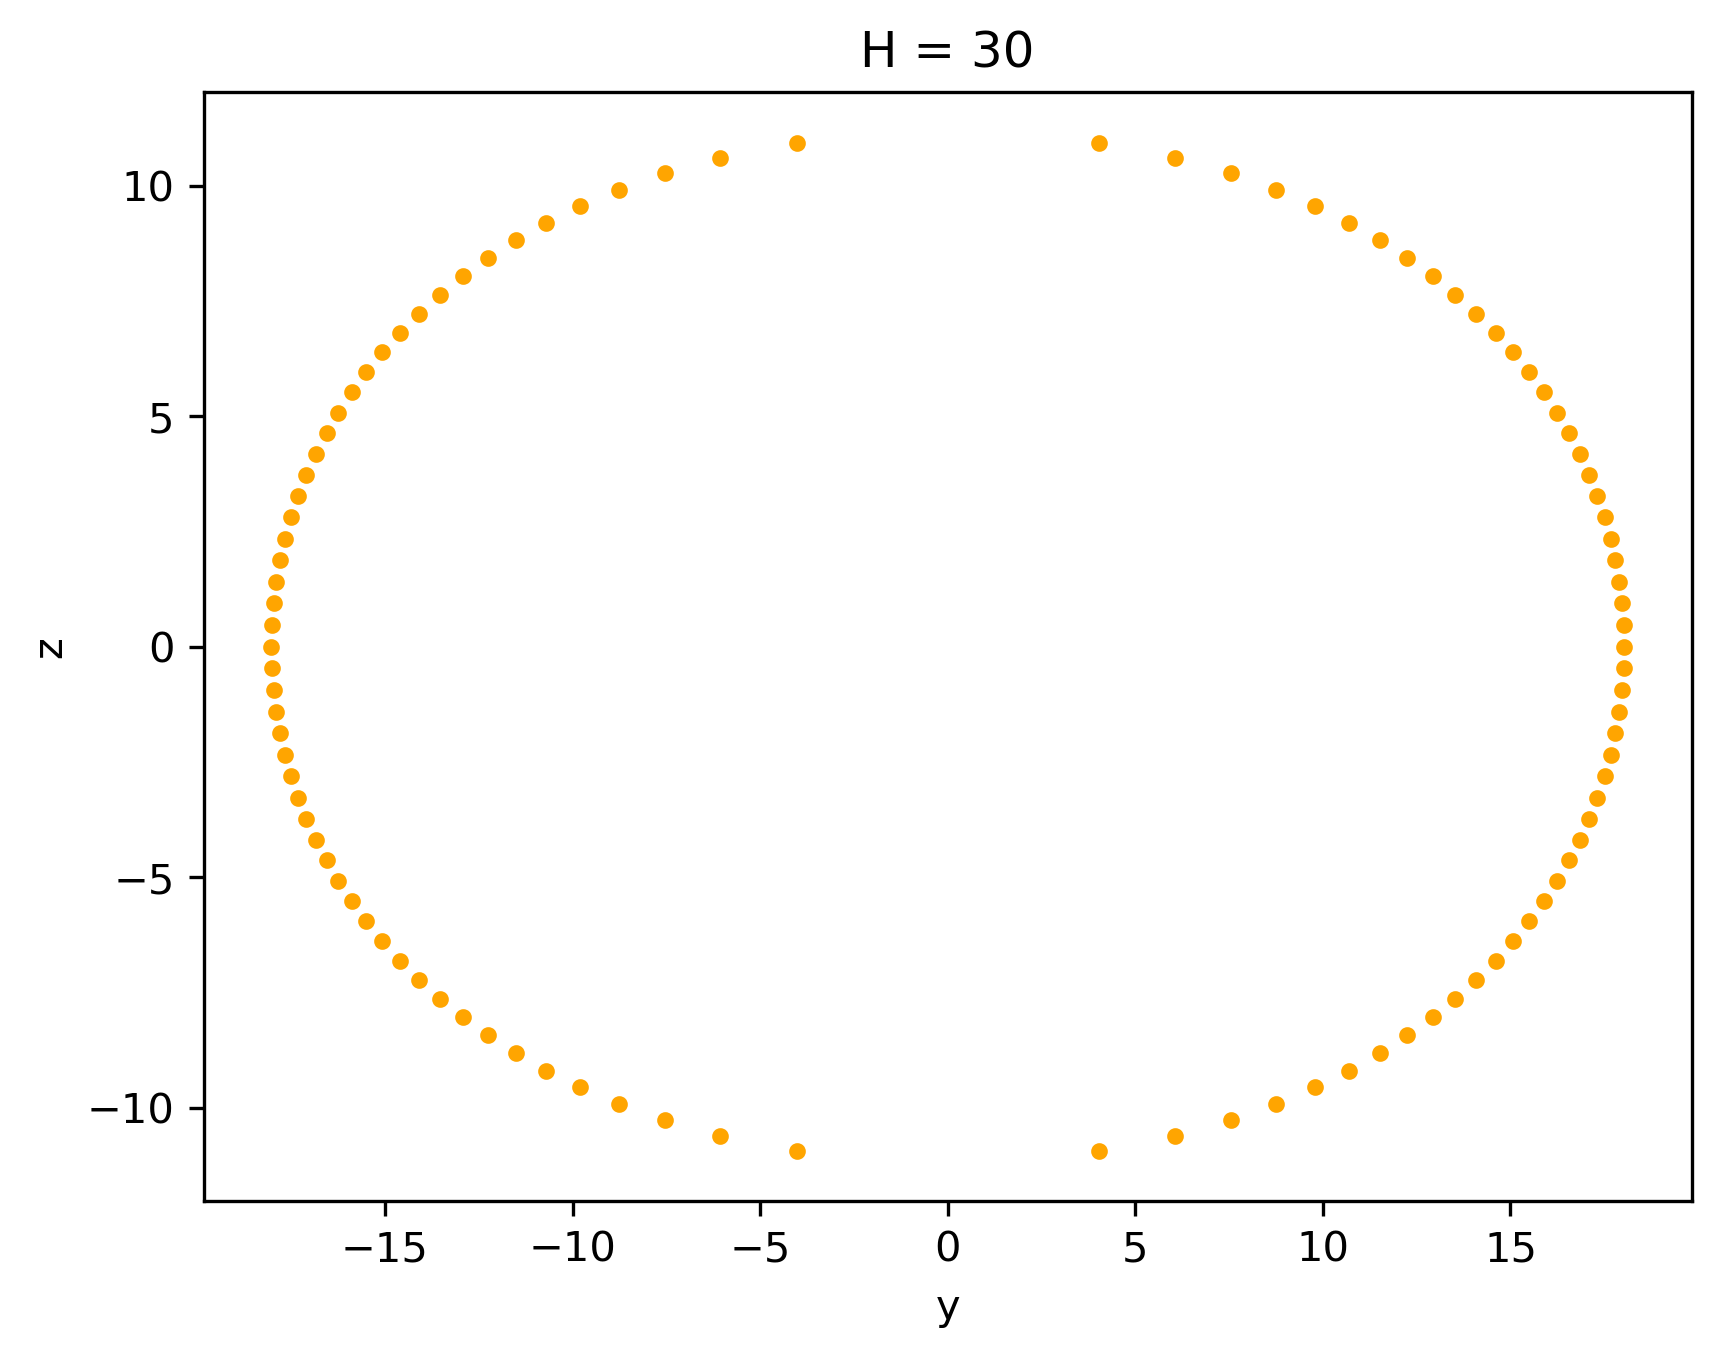
\includegraphics[scale=0.9]{TS30.png}

\caption{Сечение тора плоскость $x=35$ }
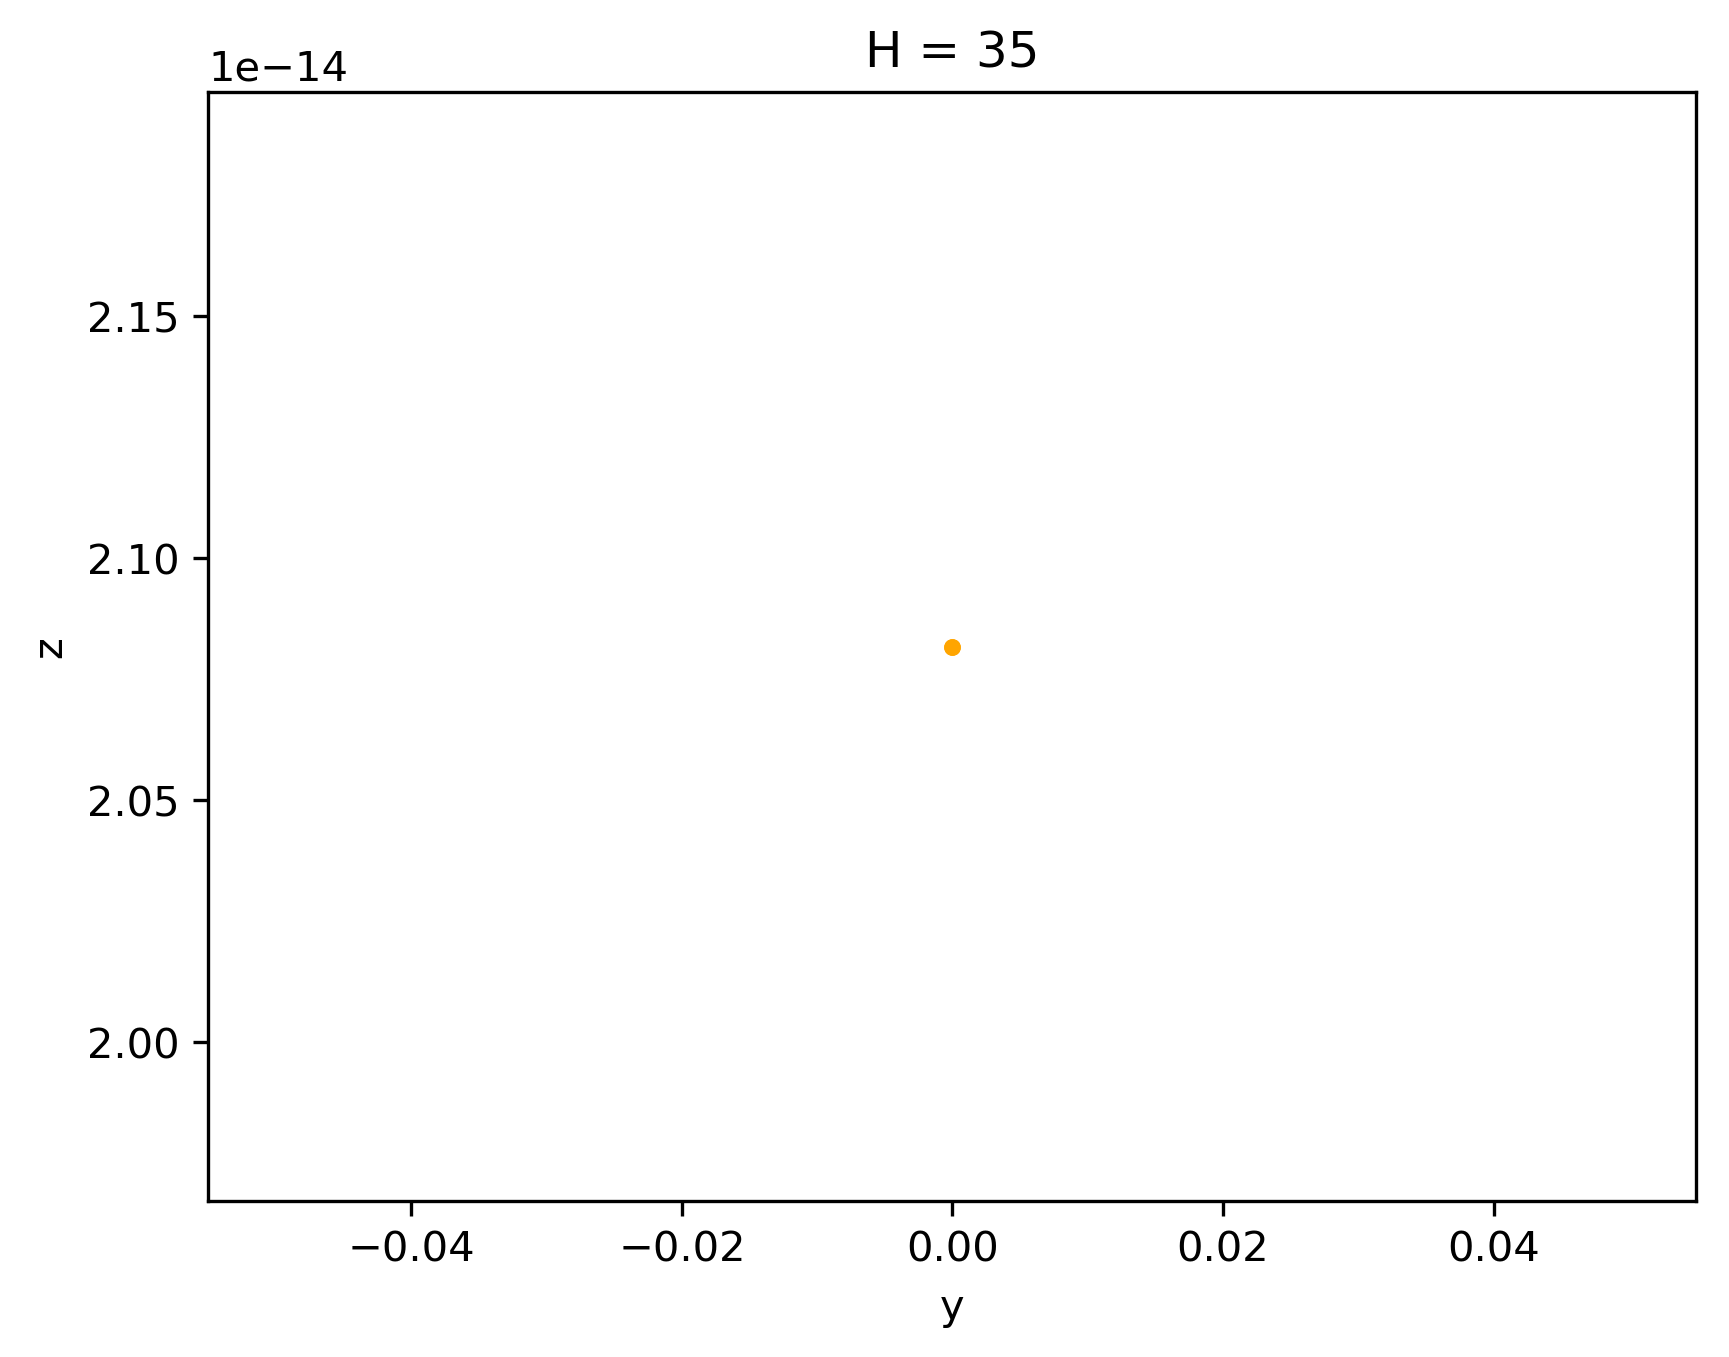
\includegraphics[scale=0.9]{TS35.png} 
\end{figure}

\begin{figure}[H]
\caption{Все сечения на одном графике }
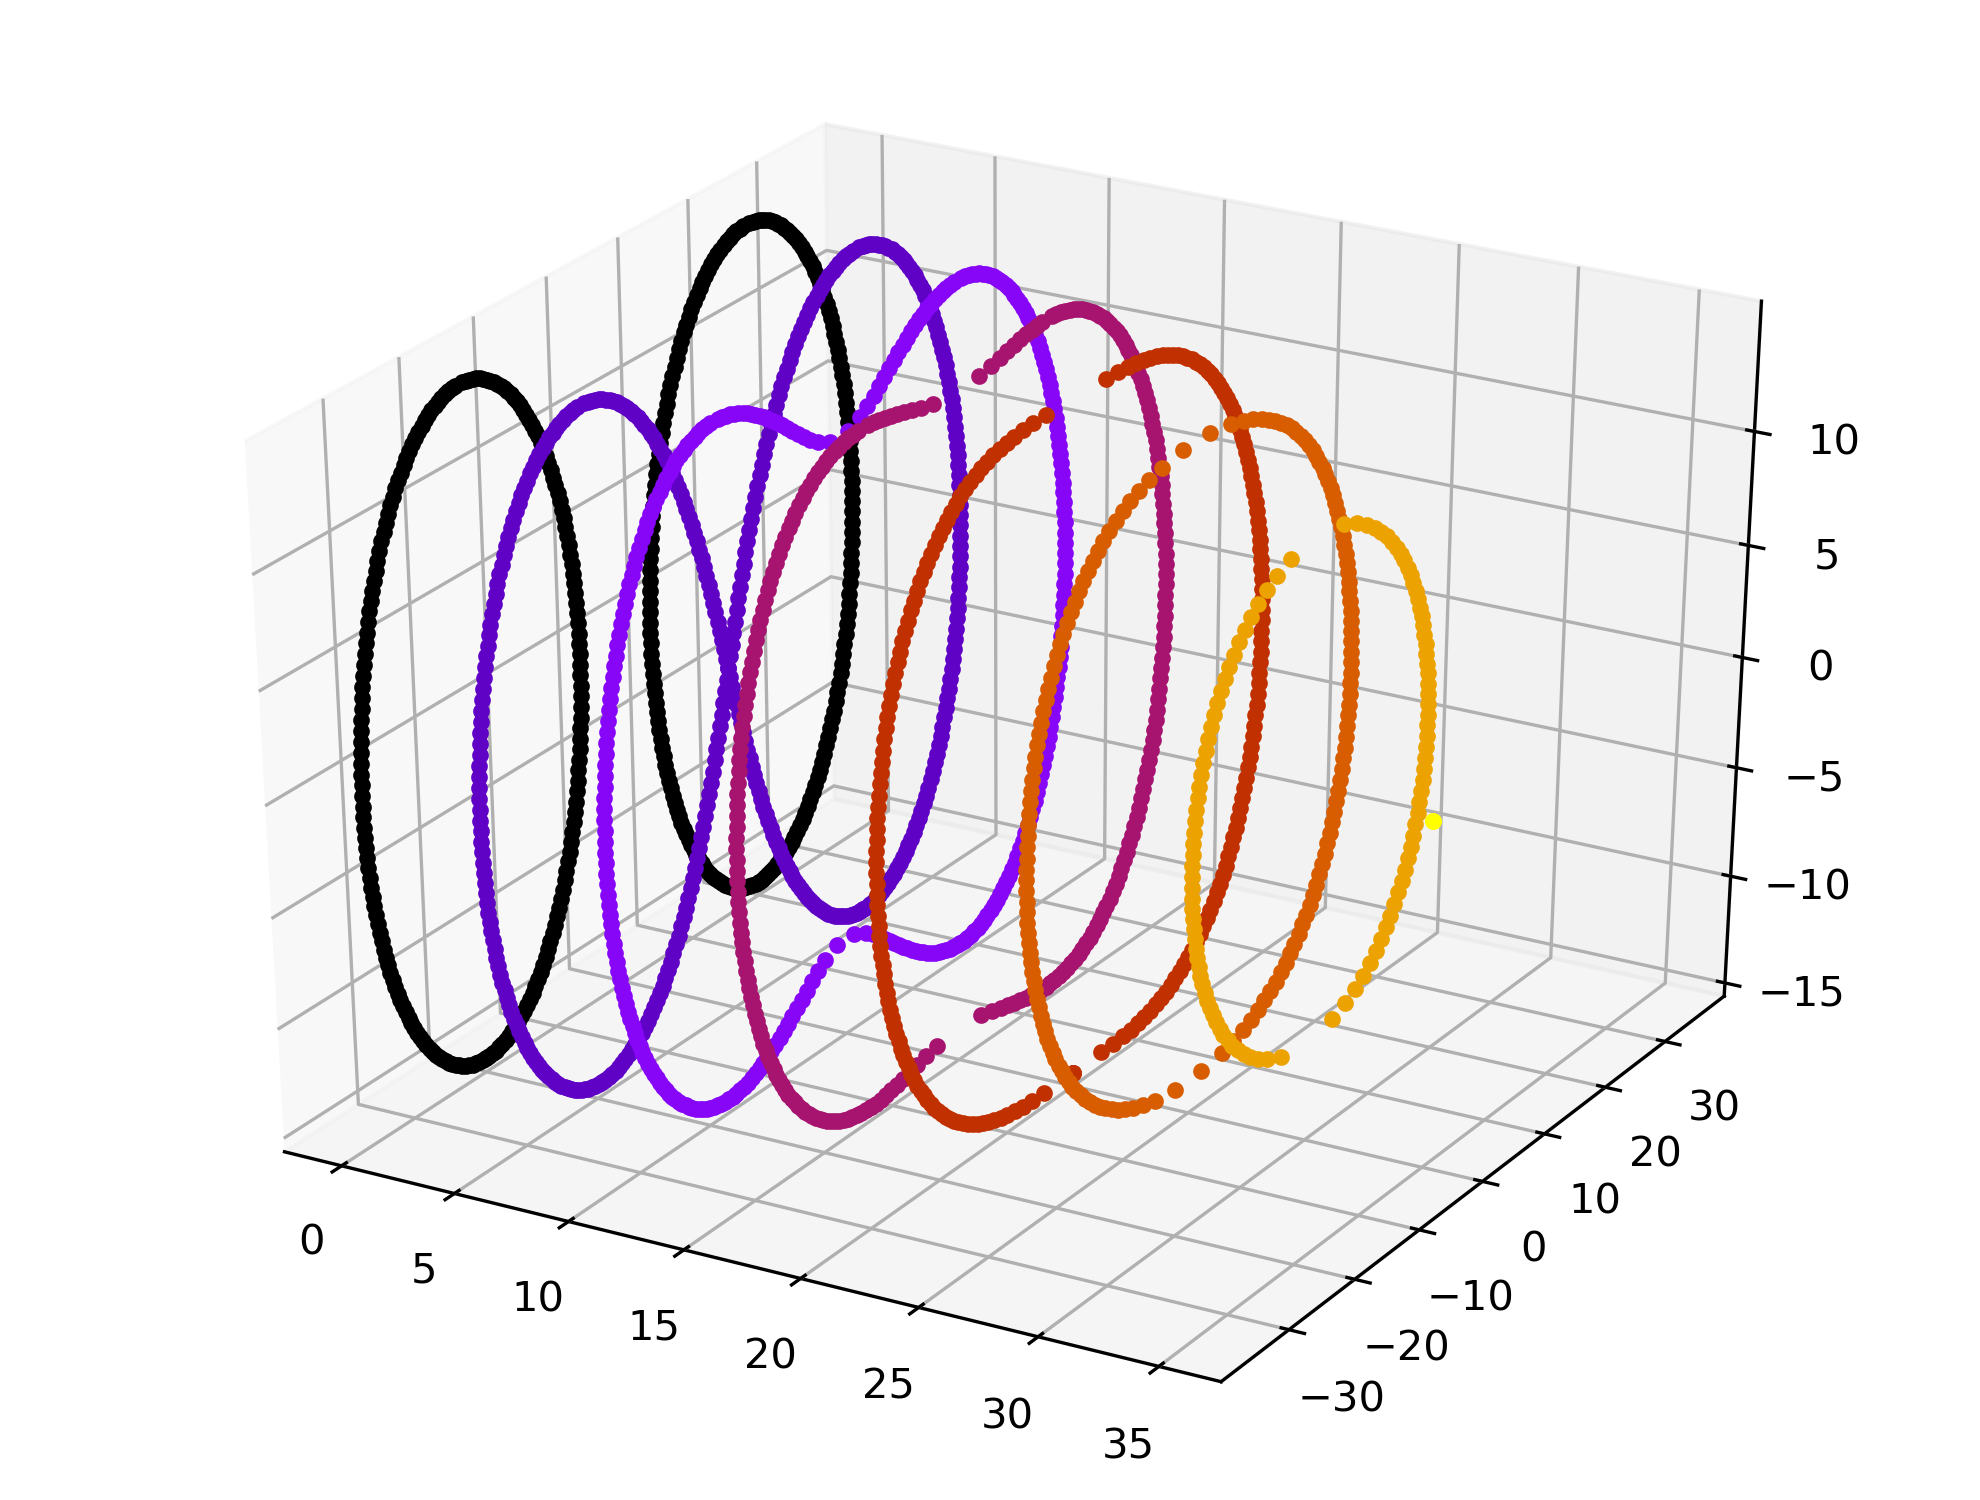
\includegraphics[scale=0.9]{TC8.png} 
\end{figure}

\newpage

\subsection{Сравнение с лемнискатой Бернулли}
Рассматривается тор со следующими характеристиками: $R=20\;\--$ радиус вращения, $r=15\;\--$ радиус образующей $c=34.$

Сечение плоскостью $x=R-r=5$ не сильно похоже на лемнискату Бернулли. 

Для их сравнения воспользуемся расстоянием Фреше: $fr = 4.2426.$


\begin{figure}[H]
\caption{Лемниската для сечения тора }
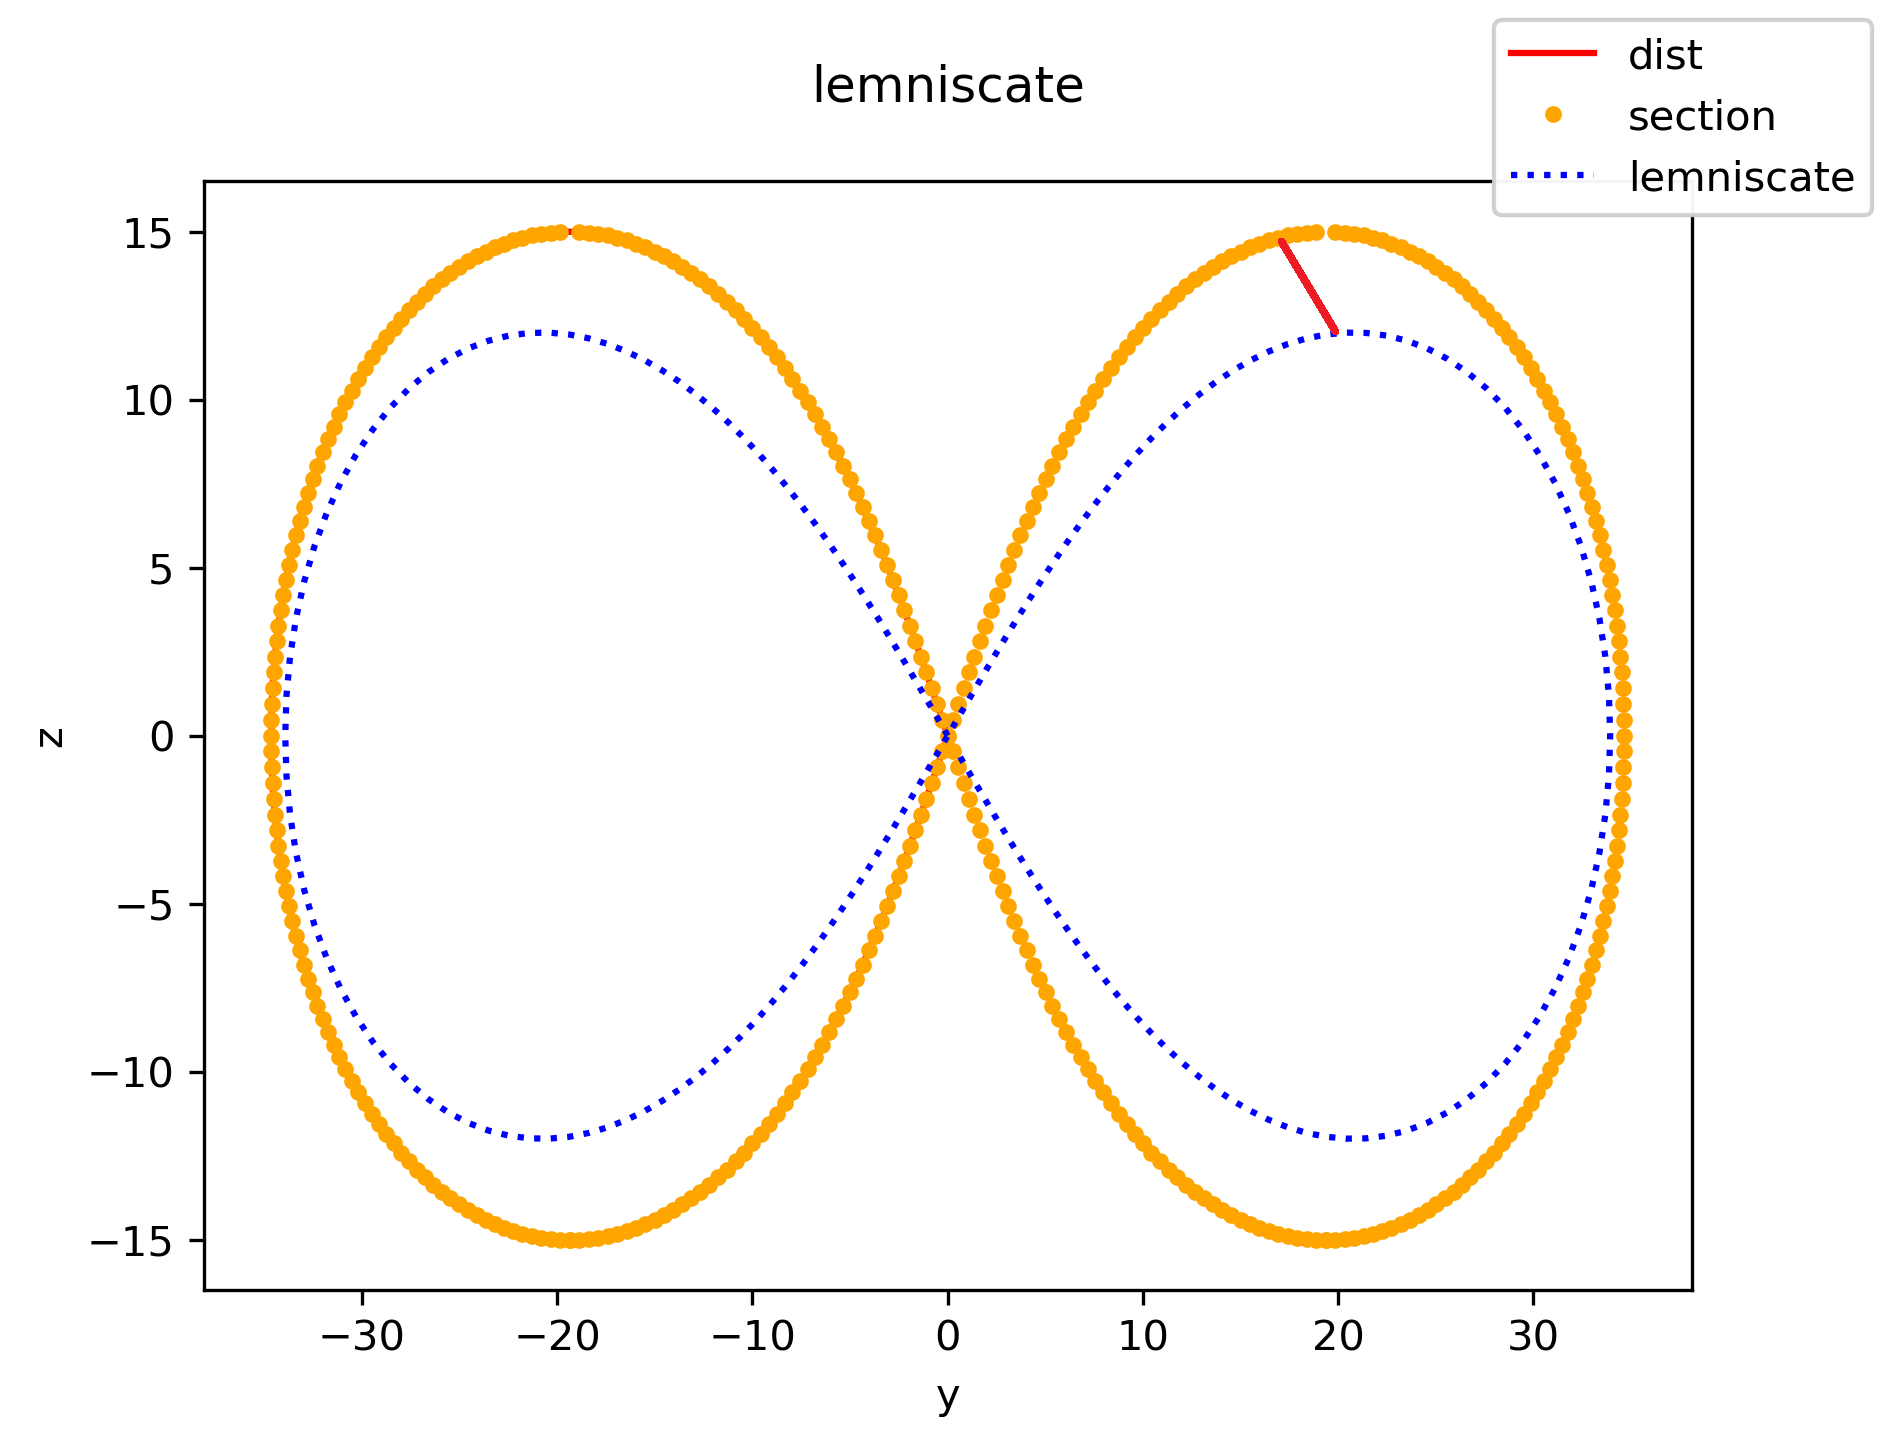
\includegraphics[scale=0.4]{lemniscate1.png} 
\end{figure}


Подберём параметры тора так, чтобы лемниската и сечение практически совпадали:
$R=10,\; r = 5,$ сечение плоскостью $x=5.$ Параметр лемнискаты $c=14.$ Расстояние Фреше $fr = 0.1938.$

\begin{figure}[H]
\caption{Лемниската практически совпадающая с сечением тора }
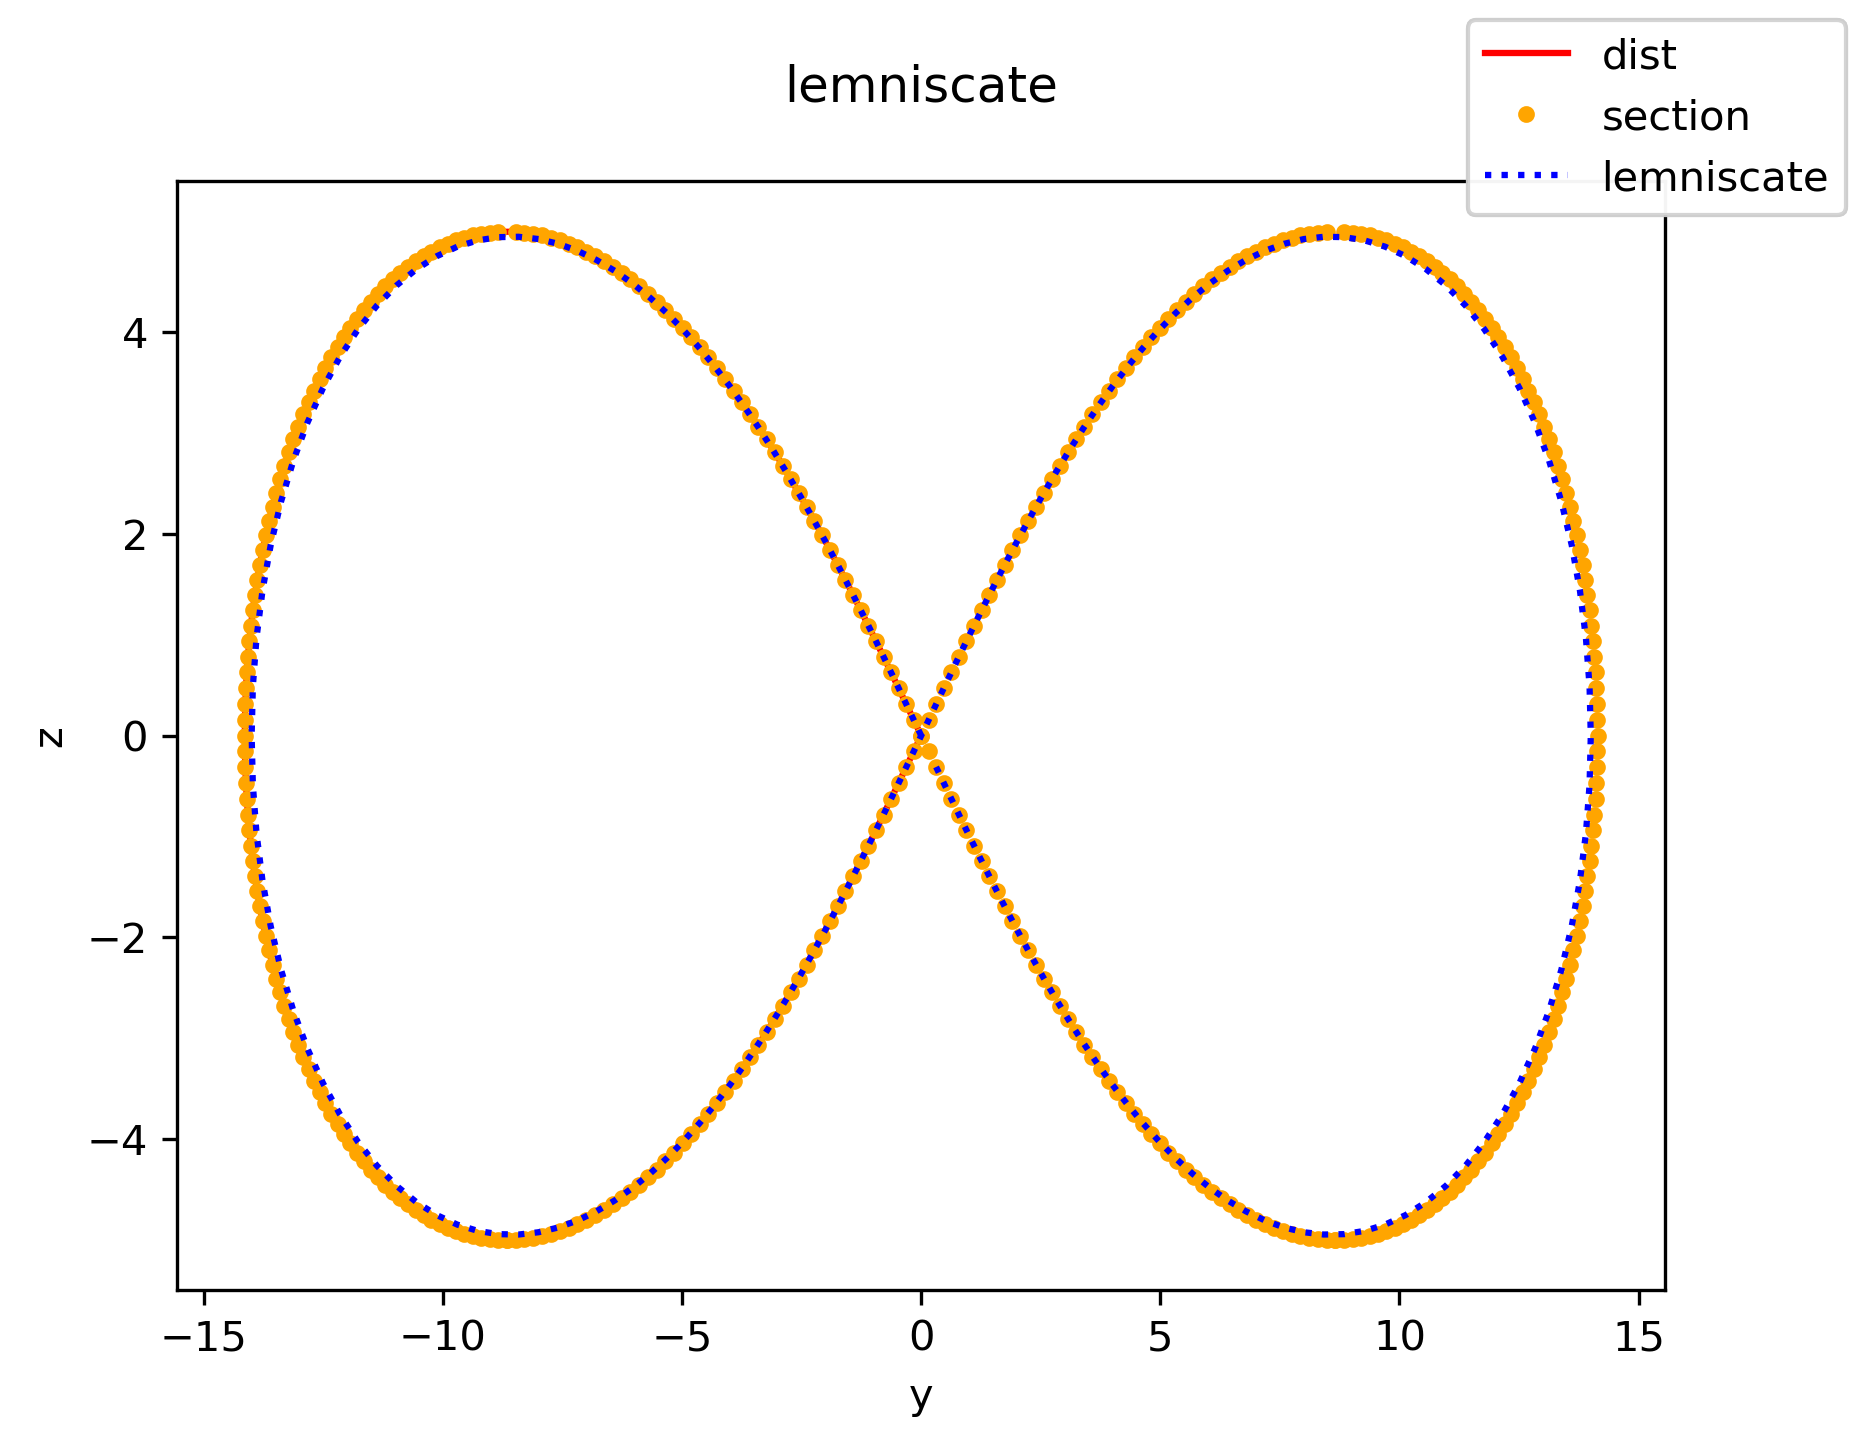
\includegraphics[scale=0.9]{lemniscate.png} 
\end{figure}

\section{Обсуждение}
По результатам видно, что общем случае сечение плоскость x=R-r действительно похоже на лемнискату Бернулли, но не совпадает с ним.

Можно подобрать параметры тора и лемнискаты так, чтобы сечение практически совпадало с лемнискатой (расстояние Фреше мало, но не равняется нулю из-за дискретизации фигур)

Для совпадения радиус образующей тора $(r)$ должен быть в $2$ раза меньше его радиуса вращения $(R).$

Параметр лемнискаты – параметр масштаба (не влияет на её форму), следовательно, от него не зависит необходимое соотношение между $r$ и $R.$

\begin{thebibliography}{}
    \bibitem{numpy}  Модуль numpy  -  https://physics.susu.ru/vorontsov/language/numpy.html
    
    \bibitem{plotlib} 
    Модуль matplotlib - https://matplotlib.org/users/index.html
    
    \bibitem{plot3}
    Модуль mpl\_toolkit - https://matplotlib.org/mpl\_toolkits/mplot3d/api.html
    
    \bibitem{source}
    Пособие к Лабораторным работам https://cloud.mail.ru/public/4ra6/5wwqBzMBC/LabPractics.pdf
\end{thebibliography}

\section{Приложения}

Код отчёта:\; \url{https://github.com/MisterProper9000/computing-complex/tree/master/Lab_2_body_of_rotation/lab2.tex}

Код лаборатрной:\; \url{https://github.com/MisterProper9000/computing-complex/blob/master/Lab_2_body_of_rotation/lab_2_code/Lab_2.py}

\lstinputlisting[language=Python]{lab2.py}

\end{document}